%%%%%%%%%%%%%%%%%%%%%%%%%%%%%%%%%%%%%
%                                   %
% Compile with XeLaTeX and biber    %
%                                   %
% Questions or comments:            %
%                                   %
% joshua dot mcneill at uga dot edu %
%                                   %
%%%%%%%%%%%%%%%%%%%%%%%%%%%%%%%%%%%%%

\documentclass{beamer}
  % Read in standard preamble (cosmetic stuff)
  %%%%%%%%%%%%%%%%%%%%%%%%%%%%%%%%%%%%%%%%%%%%%%%%%%%%%%%%%%%%%%%%
% This is a standard preamble used in for all slide documents. %
% It basically contains cosmetic settings.                     %
%                                                              %
% Joshua McNeill                                               %
% joshua dot mcneill at uga dot edu                            %
%%%%%%%%%%%%%%%%%%%%%%%%%%%%%%%%%%%%%%%%%%%%%%%%%%%%%%%%%%%%%%%%

% Beamer settings
% \usetheme{Berkeley}
\usetheme{CambridgeUS}
% \usecolortheme{dove}
% \usecolortheme{rose}
\usecolortheme{seagull}
\usefonttheme{professionalfonts}
\usefonttheme{serif}
\setbeamertemplate{bibliography item}{}

% Packages and settings
\usepackage{fontspec}
  \setmainfont{Charis SIL}
\usepackage{hyperref}
  \hypersetup{colorlinks=true,
              allcolors=blue}
\usepackage{graphicx}
  \graphicspath{{../../figures/}}
\usepackage[normalem]{ulem}
\usepackage{enumerate}

% Document information
\author{M. McNeill}
\title[FREN2001]{Français 2001}
\institute{\url{joshua.mcneill@uga.edu}}
\date{}

%% Custom commands
% Lexical items
\newcommand{\lexi}[1]{\textit{#1}}
% Gloss
\newcommand{\gloss}[1]{`#1'}
\newcommand{\tinygloss}[1]{{\tiny`#1'}}
% Orthographic representations
\newcommand{\orth}[1]{$\langle$#1$\rangle$}
% Utterances (pragmatics)
\newcommand{\uttr}[1]{`#1'}
% Sentences (pragmatics)
\newcommand{\sent}[1]{\textit{#1}}
% Base dir for definitions
\newcommand{\defs}{../definitions}


  % Packages and settings
  \usepackage{tikz}
    \usetikzlibrary{shapes.geometric, arrows}
    \tikzstyle{process} = [rectangle,
                           text centered,
                           draw=black,
                           align=center]
    \tikzstyle{arrow} = [thick,->]
  \usepackage[style=apa, backend=biber]{biblatex}
    \addbibresource{../references/References.bib}


  % Document information
  \subtitle[Speech Production]{Speech Production}

  %% Custom commands
  % Subsection/frame titles
  \newcommand{\suboneone}{Thoughts to messages}
  \newcommand{\subonetwo}{Models}
  \newcommand{\subonethree}{Extenuating factors}
  \newcommand{\subonefour}{Errors}
  \newcommand{\subonefive}{Practice}

\begin{document}
  % Read in the standard intro slides (title page and table of contents)
  %%%%%%%%%%%%%%%%%%%%%%%%%%%%%%%%%%%%%%%%%%%%%%%%%%%%%%%%%%%%%%%%
% This is a standard set of intro slides used in for all slide %
% documents. It basically contains the title page and table of %
% contents.                                                    %
%                                                              %
% Joshua McNeill                                               %
% joshua dot mcneill at uga dot edu                            %
%%%%%%%%%%%%%%%%%%%%%%%%%%%%%%%%%%%%%%%%%%%%%%%%%%%%%%%%%%%%%%%%

\begin{frame}
  \titlepage
  \tiny{Office: % Basically a variable for office hours location
Gilbert 121\\
        Office hours: % Basically a variable for office hours
 lundi, mercredi, vendredi 10:10--11:10
}
\end{frame}

\begin{frame}
  \tableofcontents[hideallsubsections]
\end{frame}

\AtBeginSection[]{
  \begin{frame}
    \tableofcontents[currentsection,
                     hideallsubsections]
  \end{frame}
}


  \section{Speech Production}
    \subsection{\suboneone}
      \begin{frame}{\suboneone}
        \begin{block}{A very general model}
          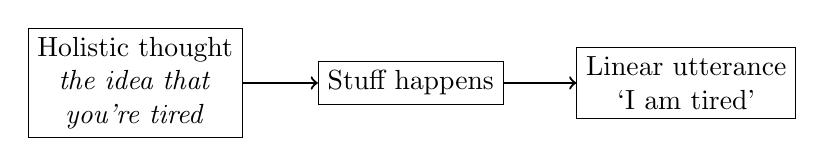
\begin{tikzpicture}[node distance=3.5cm]
            \node (holistic) [process]                    {Holistic thought \\
                                                          \emph{the idea that} \\
                                                          \emph{you're tired}};
            \node (stuff)    [process, right of=holistic] {Stuff happens};
            \node (linear)   [process, right of=stuff]    {Linear utterance \\
                                                          \uttr{I am tired}};
            \draw [arrow] (holistic) -- (stuff);
            \draw [arrow] (stuff)    -- (linear);
          \end{tikzpicture}
        \end{block}
        \begin{block}{}
          \begin{itemize}
            \item Thoughts are whole units
            \item Sentence structures and phonetic forms are produced as linearly arranged parts
          \end{itemize}
        \end{block}
      \end{frame}

    \subsection{\subonetwo}
      \begin{frame}{\subonetwo}
        \begin{block}{Two models}
          \begin{itemize}
            \item The utterance generator model \parencite{fromkin_non-anomalous_1971}
            \item \citeauthor{levelt_speaking:_1989}'s (\citeyear{levelt_speaking:_1989}) model
          \end{itemize}
        \end{block}
      \end{frame}

      \begin{frame}[t]{\subonetwo}
        \begin{block}{The utterance generator}
          Identify meaning $\rightarrow$ Select syntactic structure $\rightarrow$ Generate intonation contour $\rightarrow$ Insert content words $\rightarrow$ Insert function words \& affixes $\rightarrow$ Specify phonetic segments
        \end{block}
        \only<1>{
          \begin{block}{This is a \alert{serial model}}
            % Serial model
A type of model for speech production or processing where steps are executed one after the other

          \end{block}
        }
        \only<2>{
          \begin{block}{Example: \uttr{Peter walked down the stairs.}}
            \begin{tabular}{r @{) } l @{: } l}
              1 & Meaning     & \emph{Peter walking down the stairs in the past} \\
              2 & Structure   & [NP \_] [V \_] [P \_] [NP \_] \\
              3 & Intonation  & [NP \_] ↗[V \_] [P \_] ↘[NP \_] \\
              4 & Content     & [NP Peter] ↗[V walk] [P \_] ↘[NP stair] \\
              5 & Function    & \begin{tabular}[t]{@{} l @{}}
                                  [NP Peter] ↗[V walk-ed] [P down] \\
                                  ↘[NP the stair-s]
                                \end{tabular} \\
              6 & Phonetics   & [ˈpi.tɹ̩ ˈwɔkt ˈdaʊn ðə ˈstɛɹz]
            \end{tabular}
          \end{block}
        }
      \end{frame}

      \begin{frame}{\subonetwo}
        \begin{block}{Levelt's model}
          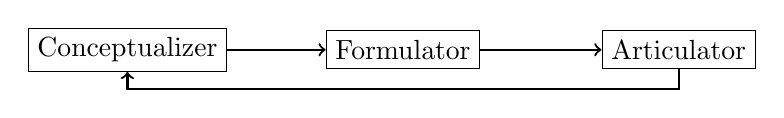
\begin{tikzpicture}[node distance=3.5cm]
            \node (concept)    [process]                   {Conceptualizer};
            \node (form)       [process, right of=concept] {Formulator};
            \node (articulate) [process, right of=form]    {Articulator};
            \draw [arrow] (concept)    -- (form);
            \draw [arrow] (form)       -- (articulate);
            \draw [arrow] (articulate) --++ (0cm, -0.5cm) -| (concept);
          \end{tikzpicture}
        \end{block}
        \begin{block}{Formulator functions}
          Grammatical encoding
          \begin{itemize}
            \item i.e., syntactic structure \& lexical expressions
          \end{itemize}
          Phonological encoding
        \end{block}
        \begin{block}{This is a \alert{parallel model}}
          % Parallel model
A type of model for speech production or processing where steps can feed back into previous steps

        \end{block}
      \end{frame}

    \subsection{\subonethree}
      \begin{frame}[t]{\subonethree}
        \begin{block}{English speech rate}
          Four syllables per second
        \end{block}
        \only<1-4>{
          \begin{columns}
            \column{0.48\linewidth}
            \begin{minipage}[c][0.6\textheight]{\linewidth}
              \begin{block}{But how does this go wrong?}
                Name the following objects as quickly as possible:
              \end{block}
              \begin{block}<4->{}
                More frequent and familiar words are produced quicker
              \end{block}
            \end{minipage}
            \column{0.48\linewidth}
            \only<2>{
            
\includegraphics[scale=0.125]{ladle.jpg}
            }
            \only<3->{
            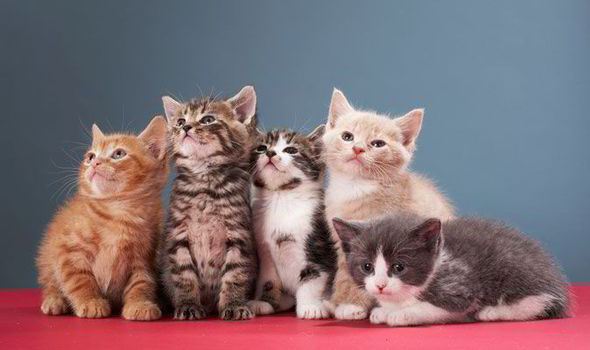
\includegraphics[scale=0.25]{cats.jpg}
            }
          \end{columns}
        }
        \only<5->{
          \begin{block}{Word length isn't important}
            Speakers start to say
            \begin{itemize}
              \item \lexi{cat} and
              \item \lexi{caterpillar}
            \end{itemize}
            equally quickly \parencite{damian_does_2010}
          \end{block}
        }
      \end{frame}

      \begin{frame}{\subonethree}
        \begin{block}{It's not just speech rate}
          \alert{Phonetic reduction}: % Phonetic reduction
When the phonetic details of a word are minimized, typically by shortening or deleting sounds

        \end{block}
        \begin{block}{How do you pronounce \lexi{probably}?}
          \uncover<2->{
            \begin{itemize}
              \item In careful speech: [ˈpɹɑ.bə.bli]?
              \item Repeated in casual speech: [ˈpɹɑ.bli]? [ˈpɹɑ.li]?
            \end{itemize}
          }
        \end{block}
        \begin{block}<3->{A side-effect}
          Repetitions also increase how quickly we access a word
        \end{block}
      \end{frame}

    \subsection{\subonefour}
      \begin{frame}{\subonefour}
        \begin{block}{}
          We use production errors to understand language better and ultimately to test production models
        \end{block}
        \begin{columns}
          \column{0.48\linewidth}
          \begin{block}{Is uttering the word \uttr{untasteful} an error?}
            \uncover<2->{
            \begin{itemize}
              \item If part of competence: No
              \item If part of performance: Yes
            \end{itemize}
            }
          \end{block}
          \column{0.48\linewidth}
          \uncover<2->{
          
\includegraphics[scale=0.125]{performance_cat.jpg}
          }
        \end{columns}
      \end{frame}

      \begin{frame}{\subonefour}
        \begin{block}{Types of production errors}
          \begin{itemize}
            \item Anticipation
            \item Perseveration
            \item Addition
            \item Deletion
            \item Metathesis
            \item Spoonerism
            \item Shifting
            \item Substitution
            \item Blending
          \end{itemize}
        \end{block}
      \end{frame}

      \begin{frame}{\subonefour}
        \begin{alertblock}{Anticipation}
          % Anticipation
When an earlier unit of an utterance is replaced by a later unit


          \begin{tabular}{r @{: } l}
            Meant & \sent{spl\alert{i}cing from one t\alert{a}pe} \\
            Said  & \uttr{spl\alert{a}cing from one t\alert{a}pe}
          \end{tabular}
        \end{alertblock}
        \begin{alertblock}{Perseveration}
          % Perseveration
When an earlier unit of an utterance is used to replace a later unit


          \begin{tabular}{r @{: } l}
            Meant & \sent{spl\alert{i}cing from one t\alert{a}pe} \\
            Said  & \uttr{spl\alert{i}cing from one t\alert{y}pe}
          \end{tabular}
        \end{alertblock}
      \end{frame}

      \begin{frame}{\subonefour}
        \begin{alertblock}{Addition}
          % Addition
When a unit has been inserted into an utterance out of nowhere


          \begin{tabular}{r @{: } l}
            Meant & \sent{spic and span} \\
            Said  & \uttr{spic and sp\alert{l}an}
          \end{tabular}
        \end{alertblock}
        \begin{alertblock}{Deletion}
          % Deletion
When a unit has been removed from an utterance


          \begin{tabular}{r @{: } l}
            Meant & \sent{his immor\alert{t}al soul} \\
            Said  & \uttr{his immoral soul}
          \end{tabular}
        \end{alertblock}
      \end{frame}

      \begin{frame}{\subonefour}
        \begin{alertblock}{Metathesis}
          % Metathesis (error)
When two units of an utterance switch places


          \begin{tabular}{r @{: } l}
            Meant & \sent{f\alert{i}ll the p\alert{oo}l} \\
            Said  & \uttr{f\alert{oo}l the p\alert{i}ll}
          \end{tabular}
        \end{alertblock}
        \begin{alertblock}{Spoonerism}
          % Spoonerism
A special type of metathesis that involves the first sounds of two different words switching


          \begin{tabular}{r @{: } l}
            Meant & \sent{\alert{f}ill the \alert{p}ool} \\
            Said  & \uttr{\alert{p}ill the \alert{f}ool}
          \end{tabular}
        \end{alertblock}
      \end{frame}

      \begin{frame}{\subonefour}
        \begin{alertblock}{Shifting}
          % Shifting
When a unit of an utterance has been moved from one location to another


          \begin{tabular}{r @{: } l}
            Meant & \sent{she decide\alert{s} to hit it} \\
            Said  & \uttr{she decide to hit\alert{s} it}
          \end{tabular}
        \end{alertblock}
        \begin{alertblock}{Substitution}
          % Substitution
When a unit of an utterance has replaced with another unit out of nowhere


          \begin{tabular}{r @{: } l}
            Meant & \sent{it's \alert{hot} in here} \\
            Said  & \uttr{it's \alert{cold} in here}
          \end{tabular}
        \end{alertblock}
        \begin{block}<2->{}
          These examples involve morphemes and words, respectively
        \end{block}
      \end{frame}

      \begin{frame}{\subonefour}
        \begin{alertblock}{Blending}
          % Blending
When two units of an utterance are merged into one unit


          \begin{tabular}{r @{: } l}
            Meant & \sent{grizzly and ghastly} \\
            Said  & \uttr{grastly}
          \end{tabular}
        \end{alertblock}
      \end{frame}

      \begin{frame}{\subonefour}
        \begin{block}{Are phonemes, morphemes, and words real?}
          Even our errors involve these units
          \begin{itemize}
            \item Why not \sent{decides to hit} $\rightarrow$ \uttr{deci to hitdes}?
          \end{itemize}
        \end{block}
        \begin{block}<2->{What about features?}
          Errors can involve just a single feature
          \begin{itemize}
            \item \sent{clear blue sky} $\rightarrow$ \uttr{glear plue sky}
          \end{itemize}
        \end{block}
      \end{frame}

      \begin{frame}{\subonefour}
        \begin{block}{Are rules real?}
          Phonotactics are adhered to in errors
          \begin{itemize}
            \item \sent{Freudian slip} $\rightarrow$ \uttr{Fleudian [ʃɹ]ip}
          \end{itemize}
          And morphological rules
          \begin{itemize}
            \item \sent{cook[t] a roast} $\rightarrow$ \uttr{roast[əd] a cook}
          \end{itemize}
        \end{block}
      \end{frame}

      \begin{frame}{\subonefour}
        \begin{block}{Are sense relations real?}
          Substitutions are often semantically related
          \begin{itemize}
            \item \sent{My thesis is too \alert{long}} $\rightarrow$ \uttr{My thesis is too \alert{short}}
            \item \sent{before the place \alert{opens}} $\rightarrow$ \uttr{Before the place \alert{closes}}
          \end{itemize}
        \end{block}
        \begin{block}<2->{Are there phonological links in speakers' mental lexicons?}
          Substitutions are often phonologically similar
          \begin{itemize}
            \item \sent{spreading like wild\alert{fire}} $\rightarrow$ \uttr{spreading like wild\alert{flowers}}
            \item \sent{I'm a \alert{contortionist}!} $\rightarrow$ \uttr{I'm an \alert{extortionist}!}
          \end{itemize}
          \alert{Malapropism}: % Malapropism
A substitution in which a word in an utterance is replaced by a similar sounding word

        \end{block}
      \end{frame}

      \begin{frame}[t]{\subonefour}
        \begin{example}
          \begin{itemize}
            \item Plural morpheme: /z/
            \item Plural allomorphs: [z], [əz], [s]
            \item \sent{\emph{[ˈmɪ.nɪ.stɹ̩\alert{z}]} in our church} $\rightarrow$ \uttr{[ˈtʃɹ̩.tʃ\alert{əz}] in our minister}
          \end{itemize}
        \end{example}
        \only<1>{
          \begin{block}{Does this support the utterance generator model?}
            \begin{itemize}
              \item (4) Insert content words $\rightarrow$ (5) Insert function words \& affixes $\rightarrow$ (6) Specify phonetic segments
            \end{itemize}
          \end{block}
        }
        \only<2>{
          \begin{block}{Does this support Levelt's model?}
            \begin{itemize}
              \item (1) Conceptualizer $\rightarrow$ (2) Formulator (\mbox{(2a) Grammatical encoding} $\rightarrow$ \mbox{(2b) Phonological encoding}) $\rightarrow$ (3) Articulator
            \end{itemize}
          \end{block}
        }
      \end{frame}

      \begin{frame}[t]{\subonefour}
        \begin{example}
          \parbox{0.48\linewidth}{
            \begin{tabular}{r l l}
              a)  & Farm  & Smoke \\
                  & Fern  & Smash \\
                  & Fat   & Small \\
                  & Smart & Fell
            \end{tabular}
          }
          \parbox{0.48\linewidth}{
            \begin{tabular}{r l l}
              b)  & Tail  & Smoke \\
                  & Term  & Smash \\
                  & Tank  & Small \\
                  & Smart & Tell
            \end{tabular}
          }
        \end{example}
        \only<-2>{
          \begin{block}{Which is more likely to yield a spoonerism? \parencite{motley_covert_1982}}
            \uncover<2->{
              (a) because \uttr{fart smell} is taboo and \uttr{tart smell} is not
              \begin{itemize}
                \item This means we check the resulting words before we utter them
              \end{itemize}
            }
          \end{block}
        }
        \only<3-4>{
          \begin{block}{Does this support the utterance generator model?}
            \uncover<4->{
              No: (6) \emph{Specify phonetic segments} has to feed back into (4) \emph{Insert content words} to avoid taboo
            }
          \end{block}
        }
        \only<5->{
          \begin{block}{Does this support Levelt's model?}
            Yes: Parallel models support feedback
          \end{block}
        }
      \end{frame}

      % Both models need to add post-articulation feedback though: we stop ourselves when we can hear ourselves mess up (Postma & Noordanus 1996)

    \subsection{\subonefive}
      \begin{frame}{\subonefive}
        \begin{block}{Try these}
          \textcite{dawson_language_2016}, chapter 9 exercises 9 and 12
        \end{block}
      \end{frame}

      \begin{frame}[allowframebreaks]{References}
        \printbibliography
      \end{frame}
\end{document}
